%%%%%%%%%%%%%%%%%%%%%%%%%%%%%%%%%%%%%%%%%
% Beamer Presentation
% LaTeX Template
% Version 1.0 (10/11/12)
%
% This template has been downloaded from:
% http://www.LaTeXTemplates.com
%
% License:
% CC BY-NC-SA 3.0 (http://creativecommons.org/licenses/by-nc-sa/3.0/)
%
%%%%%%%%%%%%%%%%%%%%%%%%%%%%%%%%%%%%%%%%%

%----------------------------------------------------------------------------------------
%	PACKAGES AND THEMES
%----------------------------------------------------------------------------------------

\documentclass{beamer}

\mode<presentation> {

% The Beamer class comes with a number of default slide themes
% which change the colors and layouts of slides. Below this is a list
% of all the themes, uncomment each in turn to see what they look like.

%\usetheme{default}
%\usetheme{AnnArbor}
%\usetheme{Antibes}
%\usetheme{Bergen}
%\usetheme{Berkeley}
%\usetheme{Berlin}
%\usetheme{Boadilla}
%\usetheme{CambridgeUS}
%\usetheme{Copenhagen}
%\usetheme{Darmstadt}
%\usetheme{Dresden}
%\usetheme{Frankfurt}
%\usetheme{Goettingen}
%\usetheme{Hannover}
%\usetheme{Ilmenau}
%\usetheme{JuanLesPins}
%\usetheme{Luebeck}
\usetheme{Madrid}
%\usetheme{Malmoe}
%\usetheme{Marburg}
%\usetheme{Montpellier}
%\usetheme{PaloAlto}
%\usetheme{Pittsburgh}
%\usetheme{Rochester}
%\usetheme{Singapore}
%\usetheme{Szeged}
%\usetheme{Warsaw}

% As well as themes, the Beamer class has a number of color themes
% for any slide theme. Uncomment each of these in turn to see how it
% changes the colors of your current slide theme.

%\usecolortheme{albatross}
%\usecolortheme{beaver}
%\usecolortheme{beetle}
%\usecolortheme{crane}
%\usecolortheme{dolphin}
%\usecolortheme{dove}
%\usecolortheme{fly}
%\usecolortheme{lily}
%\usecolortheme{orchid}
%\usecolortheme{rose}
%\usecolortheme{seagull}
%\usecolortheme{seahorse}
%\usecolortheme{whale}
%\usecolortheme{wolverine}

%\setbeamertemplate{footline} % To remove the footer line in all slides uncomment this line
%\setbeamertemplate{footline}[page number] % To replace the footer line in all slides with a simple slide count uncomment this line

%\setbeamertemplate{navigation symbols}{} % To remove the navigation symbols from the bottom of all slides uncomment this line
}

\usepackage{graphicx} % Allows including images
\usepackage{booktabs} % Allows the use of \toprule, \midrule and \bottomrule in tables
\usepackage[slovene]{babel} % slovenske nastavitve (naslovi, deljenje besed ...)
\usepackage[T1]{fontenc}    % font encoding; T1 podpira slovenščino
\usepackage[utf8]{inputenc}
\usepackage{subcaption}

%----------------------------------------------------------------------------------------
%	TITLE PAGE
%----------------------------------------------------------------------------------------

\title[Markov switching]{Electricity price forecasting using Markov regime switching model} % The short title appears at the bottom of every slide, the full title is only on the title page

\author{Rok Ivanšek} % Your name
\institute[University of Ljubljana] % Your institution as it will appear on the bottom of every slide, may be shorthand to save space
{
Faculty of Mathematics and Physics \\ % Your institution for the title page
\medskip
%\textit{•} % Your email address
}
\date{\today} % Date, can be changed to a custom date

\begin{document}

\begin{frame}
\titlepage % Print the title page as the first slide
\end{frame}

\begin{frame}
\frametitle{Overview} % Table of contents slide, comment this block out to remove it
\tableofcontents % Throughout your presentation, if you choose to use \section{} and \subsection{} commands, these will automatically be printed on this slide as an overview of your presentation
\end{frame}

%----------------------------------------------------------------------------------------
%	PRESENTATION SLIDES
%----------------------------------------------------------------------------------------

\section{Introduction}

\begin{frame}
\frametitle{Electricity price forecasting using Markov regime switching model}

\begin{itemize}
\item Take publicly available data on electricity prices
\item Pre-process it (deseasonalize, average, split to train and test)
\item Choose an appropriate regime switching model
\item Fit the model using EM algorithm
\item Run a simulation and try to predict test data
\item Measure performance
\end{itemize}

\end{frame}

%------------------------------------------------
\section{Data} % Sections can be created in order to organize your presentation into discrete blocks, all sections and subsections are automatically printed in the table of contents as an overview of the talk
%------------------------------------------------

%\subsection{Subsection Example} % A subsection can be created just before a set of slides with a common theme to further break down your presentation into chunks

\begin{frame}
\frametitle{Electricity price data}

\begin{itemize}
\item The data is publicly available
\item Is influenced by seasons, has a weekly trend
\item Deseasonalizing needed
\item Exhibits random periods when prices spike
\end{itemize}

\begin{figure}
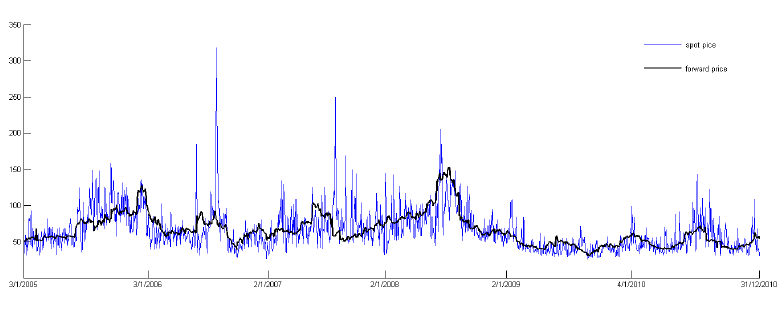
\includegraphics[width=0.8\linewidth]{electricity_price.jpg}
\end{figure}

\end{frame}

\begin{frame}
\frametitle{Electricity price data}

\begin{figure}
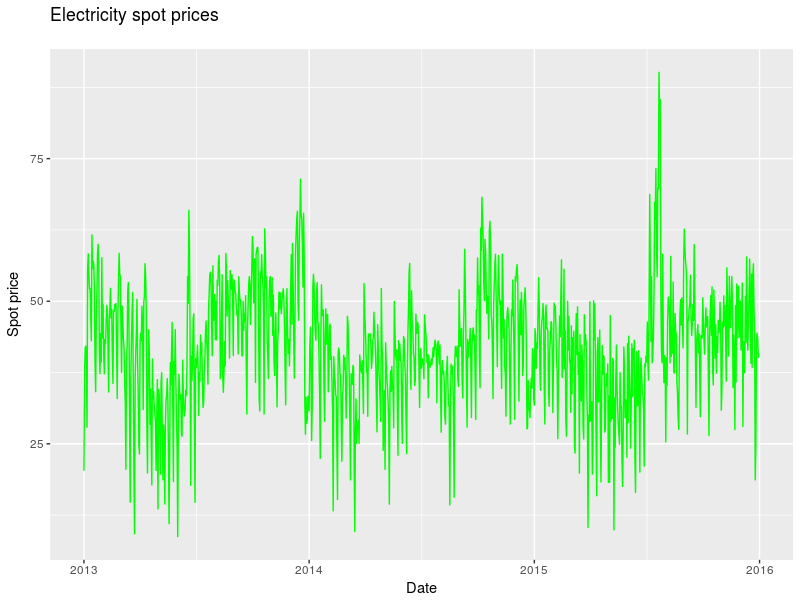
\includegraphics[width=0.85\linewidth]{dnevne_cene_2013_2015.png}
\end{figure}

\end{frame}

\begin{frame}
\frametitle{Electricity price data}

\begin{figure}
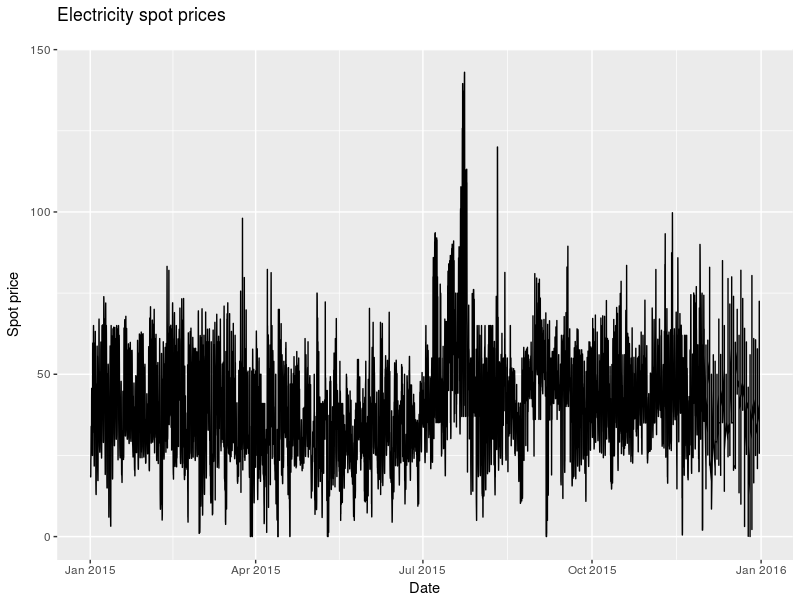
\includegraphics[width=0.85\linewidth]{hourly_data.png}
\end{figure}

\end{frame}

%------------------------------------------------
\section{Deseasonalizing}
%------------------------------------------------

\begin{frame}
\frametitle{Deseasonalizing}
\begin{itemize}
\item The focus in a different project
\item I used a preexisting STL function in R
\item It detects trend and seasons in your time series data
\item After subtracting trend and seasons you are left with the stochastic part of your process
\end{itemize}
\end{frame}

\begin{frame}
\frametitle{Deseasonalizing}

\begin{figure}
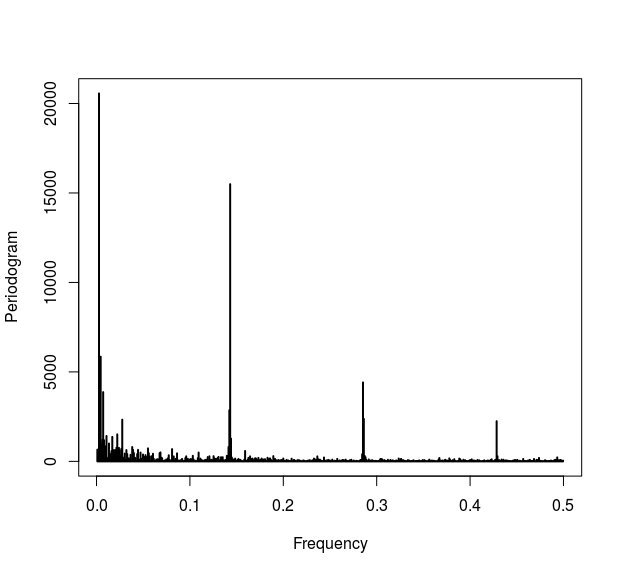
\includegraphics[width=0.7\linewidth]{periodogram.png}
\end{figure}

\end{frame}

\begin{frame}
\frametitle{Deseasonalizing}

\begin{figure}
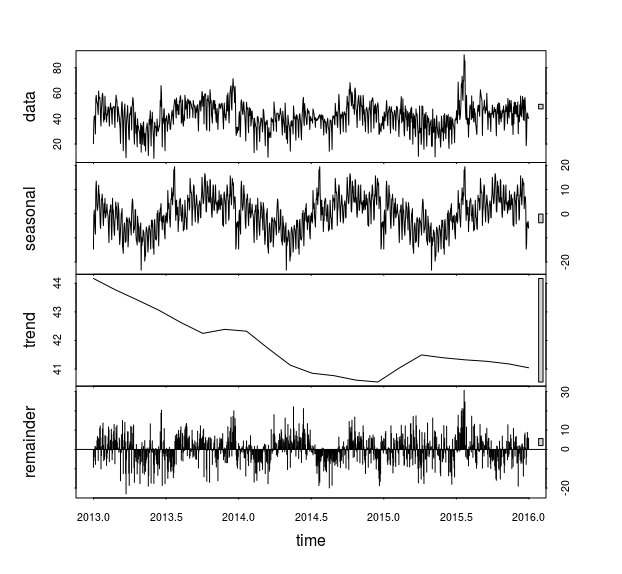
\includegraphics[width=0.7\linewidth]{stl_plot.png}
\end{figure}

\end{frame}

\begin{frame}
\frametitle{Deseasonalizing}

\begin{figure}
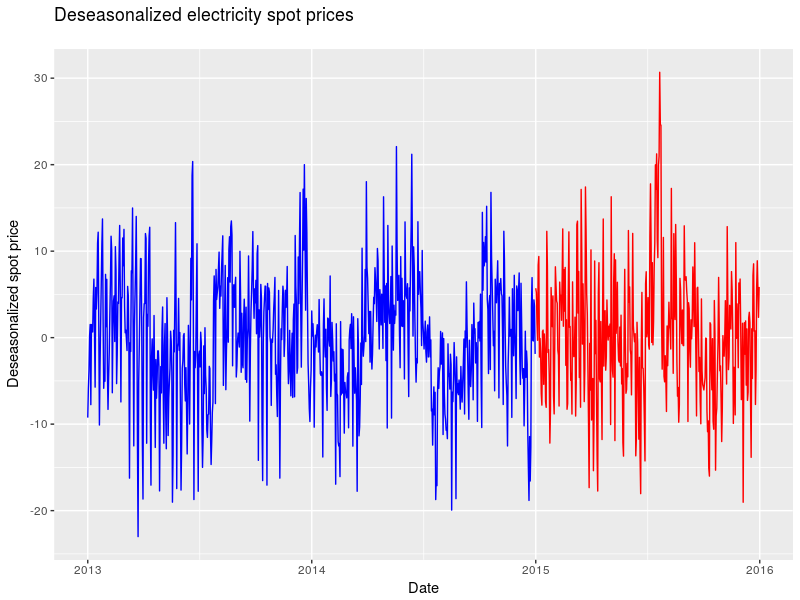
\includegraphics[width=0.85\linewidth]{deseasonalized_data.png}
\end{figure}

\end{frame}

%------------------------------------------------
\section{Markov switching model}
%------------------------------------------------

\begin{frame}
\frametitle{Markov switching model}
\begin{itemize}
\item What is a Markov switching model?
\item Motivation for using it in electricity prices modeling
\item Our data does not show clear signs of base an spike regimes
\item We can still use it
\item How do we use it?
\item How do we fit it to the data?
\end{itemize}
\end{frame}

%------------------------------------------------
\section{EM Algorithm}
%------------------------------------------------

\begin{frame}
\frametitle{EM Algorithm}
\begin{itemize}
\item What kind of Markov switching model was used.
\item What parameters did I have to fit.
\item EM Algorithm is iterative and gradually improves parameters using likelihood
\item Implementing this was by far the most difficult part of the project
\item Managed to do it by following an example from Erik Kole
\item It converged nicely and fitted the parameters on my data
\end{itemize}
The final parameters:

\begin{itemize}
\item $\mu_{0} = 3.21, \sigma_{0} = 6.20$
\item $\mu_{1} = -5.16, \sigma_{1} = 5.59$
\item $p_{00} = 0.97, p_{11} = 0.96$
\item $\xi \approx 0$
\end{itemize}


\end{frame}

%------------------------------------------------

%------------------------------------------------
\section{Simulation}
%------------------------------------------------

\begin{frame}
\frametitle{Simulation}

\begin{figure}
\centering
   \begin{subfigure}[b]{0.7\textwidth}
   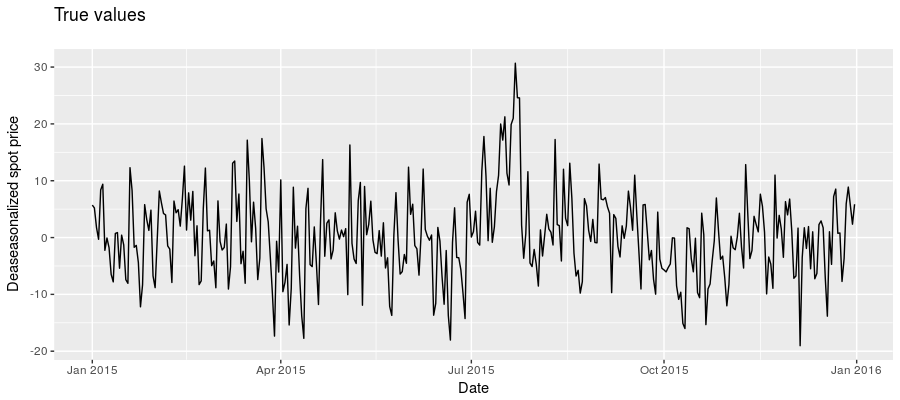
\includegraphics[width=1\linewidth]{true.png}
   \label{fig:Ng1} 
\end{subfigure}

\begin{subfigure}[b]{0.7\textwidth}
   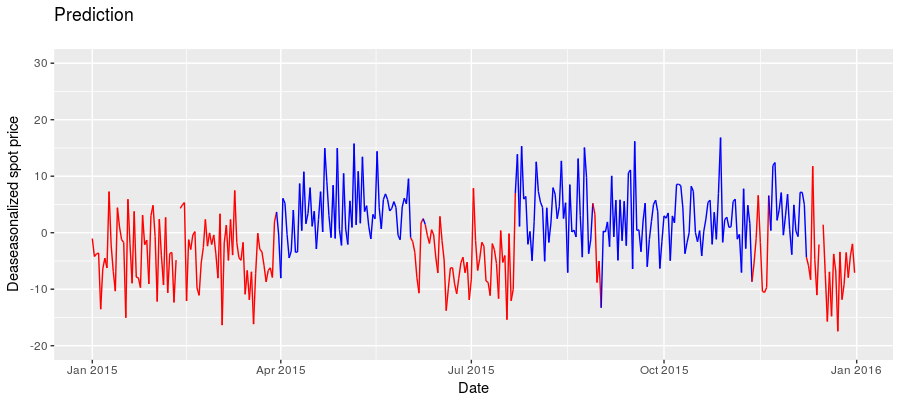
\includegraphics[width=1\linewidth]{prediction.png}
   \label{fig:Ng2}
\end{subfigure}

\end{figure}
\end{frame}

%------------------------------------------------

%------------------------------------------------
\section{Measuring performance}
%------------------------------------------------


\begin{frame}
\frametitle{Measuring performance}

\begin{itemize}
\item 20 simulations:
\item RMSE: $\mu = 10.32, \sigma = 0.44$
\item MAPE: $\mu = 29, \sigma = 1.22$
\item 1000 simulations:
\item RMSE: $\mu = 10.36, \sigma = 0.43$
\item MAPE: $\mu = 29.39, \sigma = 1.21$
\item 10000 simulations:
\item RMSE: $\mu = 10.36, \sigma = 0.43$
\item MAPE: $\mu = 29.35, \sigma = 1.27$
\end{itemize}


\end{frame}

%------------------------------------------------

\begin{frame}
\frametitle{References}
\footnotesize{
\begin{thebibliography}{99} % Beamer does not support BibTeX so references must be inserted manually as below
\bibitem[]{p1} Bierbrauer, Michael, Stefan Trück, and Rafał Weron.
\newblock Modeling electricity prices with regime switching models.
\newblock Computational Science-ICCS 2004 (2004)

\bibitem[]{p1} \url{http://prac.im.pwr.wroc.pl/~hugo/publ/BierbrauerTrueckRWeron04_ICCS.pdf}

\bibitem[]{p1} \url{http://rstudio-pubs-static.s3.amazonaws.com/1001_3177e85f5e4840be840c84452780db52.html}

\bibitem[]{p1} \url{https://personal.eur.nl/kole/rsexample.pdf}

\bibitem[]{p1} \url{https://www.r-bloggers.com/time-series-decomposition/}

\bibitem[]{p1} \url{https://anomaly.io/seasonal-trend-decomposition-in-r/}

\bibitem[]{p1} \url{https://anomaly.io/detect-seasonality-using-fourier-transform-r/}

\end{thebibliography}
}
\end{frame}

\begin{frame}
\Huge{\centerline{The End}}
\end{frame}

%----------------------------------------------------------------------------------------

\end{document}